% EcoExplain-VLM — 5 slides (pages 1, 2, 8, 9, 10 from full deck)
% Compile: cd slides && pdflatex prof_progress.tex
\documentclass[aspectratio=169,10pt]{beamer}
\usetheme{Madrid}
\usecolortheme{default}
\setbeamertemplate{navigation symbols}{}
\setbeamertemplate{footline}[frame number]

\usepackage{graphicx}
\usepackage{booktabs}
\usepackage{xcolor}
\usepackage{tikz}
\usetikzlibrary{arrows.meta, positioning}

\definecolor{donegreen}{RGB}{34,120,60}

\newcommand{\pctbar}[1]{%
  \begin{tikzpicture}[baseline=-0.5ex]
    \fill[gray!20] (0,0) rectangle (3.2,0.28);
    \fill[donegreen!70] (0,0) rectangle (#1/100*3.2,0.28);
  \end{tikzpicture}%
}

\title{EcoExplain-VLM}
\subtitle{Progress Report --- Kanha Tiger Reserve (366 patches)}
\author{Vaibhav}
\date{September 2026}

\begin{document}

% ===== Page 1 ================================================================
\begin{frame}{Project objective}
  \textbf{Central research question:}\\
  \emph{Can a vision-language model correctly classify forest vegetation change and
  generate explanations grounded in multimodal remote-sensing and climate evidence?}

  \vspace{0.5em}
  \begin{columns}[T,onlytextwidth]
    \column{0.55\textwidth}
    \textbf{What we are building}
    \begin{itemize}
      \item A \textbf{benchmark dataset} (not a new RS classifier)
      \item \textbf{366} matched before/after forest patches
      \item \textbf{Five-source evidence cube} per patch
      \item \textbf{Condition C} evaluation --- VLM sees \emph{all} sensors + masks + boxes
      \item Explanations tied to bounding boxes on 512$\times$512 images
    \end{itemize}

    \column{0.42\textwidth}
    \textbf{Study design}
    \begin{itemize}\footnotesize
      \item \textbf{Site:} Kanha Tiger Reserve
      \item \textbf{T0:} Jan--Feb 2022 \quad \textbf{T1:} Jan--Feb 2023
      \item \textbf{Patch size:} $\sim$640\,m
      \item \textbf{Classes:} stable / decline / increase
      \item \textbf{Privacy:} no lat/lon in VLM JSON
    \end{itemize}
  \end{columns}
\end{frame}

% ===== Page 2 ================================================================
\begin{frame}{Overall project completion: \texorpdfstring{$\sim$}{~}52\%}
  \small
  \begin{tabular}{@{}lcccl@{}}
    \toprule
    \textbf{Module} & \textbf{Weight} & \textbf{Done} & \textbf{Bar} & \textbf{Status} \\
    \midrule
    1.\ Data engineering        & 35\% & $\sim$95\% & \pctbar{95} & Essentially complete \\
    2.\ Dataset packaging     & 10\% & $\sim$90\% & \pctbar{90} & 366 Condition C cards \\
    3.\ Labels \& eval protocol & 15\% & $\sim$25\% & \pctbar{25} & candidate\_class only \\
    4.\ Explanations (Ollama) &  5\% & $\sim$30\% & \pctbar{30} & 366 fallback templates \\
    5.\ VLM experiments       & 25\% &  $\sim$0\% & \pctbar{0}  & Not started \\
    6.\ Results \& thesis     & 10\% & $\sim$25\% & \pctbar{25} & Mid-review deck only \\
    \midrule
    \textbf{Total project}    & 100\% & \textbf{$\sim$52\%} & & \\
    \bottomrule
  \end{tabular}

  \vspace{0.5em}
  \begin{block}{Key message}
    \textbf{Data engineering + dataset packaging are done.}\\
    Remaining: labels/eval splits, optional Ollama captions, VLM experiments.
  \end{block}
\end{frame}

% ===== Page 8 ================================================================
\begin{frame}{Condition C: every data source in each evidence card}
  \small
  \textbf{Condition C only} --- VLM receives the complete multimodal card.

  \vspace{0.25em}
  \begin{tabular}{@{}llp{5.8cm}@{}}
    \toprule
    \textbf{JSON block} & \textbf{Sensor} & \textbf{Contents per patch} \\
    \midrule
    \texttt{images}           & Sentinel-2 RGB     & T0 + T1 natural-color 512$\times$512 JPG \\
    \texttt{sentinel2}        & Sentinel-2         & 10 optical bands + NDVI/EVI/NDMI/NBR \\
    \texttt{sentinel1}        & Sentinel-1 SAR     & VV, VH (T0 + T1) \\
    \texttt{chirps}           & CHIRPS             & Rainfall mm (T0 + T1) \\
    \texttt{era5\_land}       & ERA5-Land          & Temp + soil-moisture anomalies \\
    \texttt{dem}              & NASADEM            & Elevation, slope, aspect \\
    \texttt{evidence}         & Derived            & $\Delta$NDVI, $\Delta$NBR + Otsu masks \\
    \texttt{triplets}         & Spatial GT         & Bbox + disturbance type + severity \\
    \texttt{explanation}      & Caption            & Ground-truth text \\
    \bottomrule
  \end{tabular}

  \vspace{0.3em}
  \textbf{Pipeline:} Notebook 01 (export) $\rightarrow$ 02 (DIP/boxes) $\rightarrow$ 03 (\texttt{dataset.jsonl}).
\end{frame}

% ===== Page 9 ================================================================
\begin{frame}{Repository map: what to show live}
  \begin{columns}[T,onlytextwidth]
    \column{0.50\textwidth}
    \small
    \texttt{ecoexplain\_vlm\_dataset/}
    \begin{itemize}\footnotesize
      \item \texttt{dataset.jsonl} --- open 1 record
      \item \texttt{data/preview\_chips/} --- visual QA
      \item \texttt{data/raw\_tiffs/} --- 15 files/patch
      \item \texttt{data/processed\_images/} --- JPGs + tensors
      \item \texttt{data/evidence\_masks/} --- Otsu masks
      \item \texttt{results/} --- validation reports
      \item \texttt{notebooks/01,02,03} --- pipeline
    \end{itemize}

    \textbf{Demo order:} JSONL $\rightarrow$ previews $\rightarrow$ notebook 02 $\rightarrow$ validation JSON.

    \column{0.48\textwidth}
    \centering
    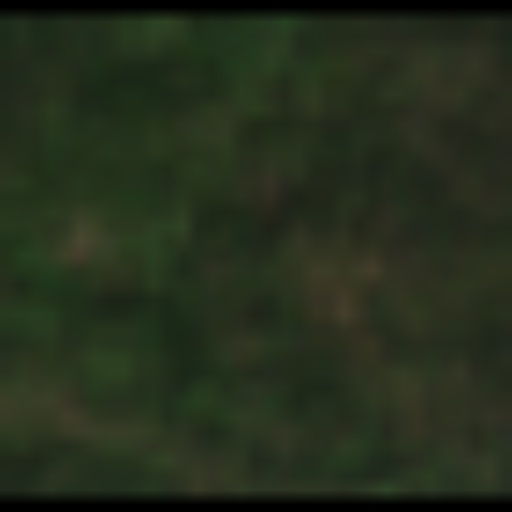
\includegraphics[width=0.48\linewidth]{figures/p00000_T0.jpg}\hfill
    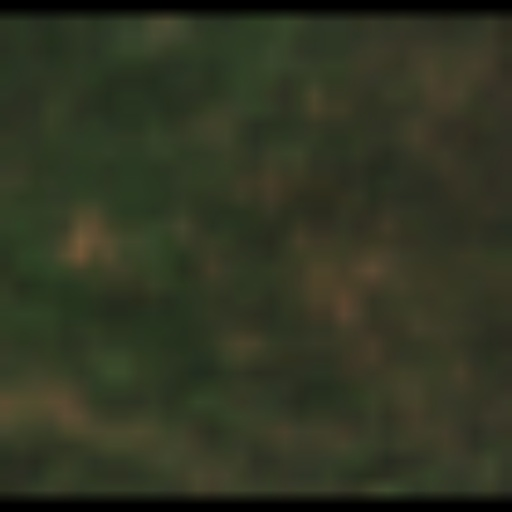
\includegraphics[width=0.48\linewidth]{figures/p00000_T1.jpg}\\
    {\scriptsize T0 (2022) \hspace{3em} T1 (2023) --- Sentinel-2 RGB, not SAR}\\[0.35em]
    
\includegraphics[width=0.48\linewidth]{figures/p00052_T0.jpg}\hfill
    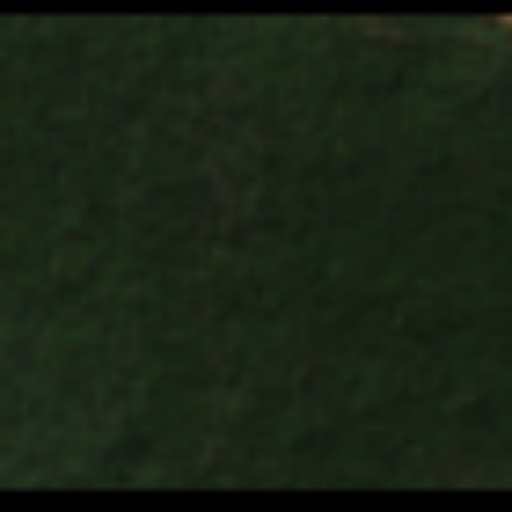
\includegraphics[width=0.48\linewidth]{figures/p01289_T0.jpg}\\
    {\scriptsize Sample chips (optical true color)}
  \end{columns}
\end{frame}

% ===== Page 10 ===============================================================
\begin{frame}{Purple-color issue, validation, and next steps}
  \begin{columns}[T,onlytextwidth]
    \column{0.40\textwidth}
    \textbf{Why purple appeared}
    \begin{itemize}\footnotesize
      \item \textbf{S2 RGB} chips, not VV/VH SAR
      \item Per-band stretch on small chips $\rightarrow$ false color
      \item \textbf{Fix:} fixed reflectance window (\texttt{vmax=0.22})
    \end{itemize}

    \vspace{0.25em}
    \textbf{Validation}
    \begin{itemize}\footnotesize
      \item 366/366 GeoTIFFs, 366 JSONL rows
      \item Preflight: \textbf{READY TO SCALE}
    \end{itemize}

    \column{0.58\textwidth}
    \centering
    \begin{tabular}{@{}c@{\hspace{0.3em}}c@{}}
      
\includegraphics[width=0.44\linewidth]{figures/purple_wrong_stretch.jpg} &
      
\includegraphics[width=0.44\linewidth]{figures/natural_correct_stretch.jpg} \\
      \scriptsize Wrong stretch (optical) & \scriptsize Correct (pipeline) \\
    \end{tabular}

    \vspace{0.35em}
    \textbf{Next:} train/dev/test splits $\rightarrow$ Condition C VLM experiments.
  \end{columns}
\end{frame}

\end{document}
